\documentclass[a4paper,12pt]{article}

% Paquetes básicos
\usepackage[utf8]{inputenc}
\usepackage[T1]{fontenc}
\usepackage[spanish]{babel}
\usepackage{graphicx}
\usepackage{xcolor}
\usepackage{lipsum}
\usepackage{geometry}
\geometry{top=3cm, bottom=3cm, left=2.5cm, right=2.5cm}

% Paquetes para diseño
\usepackage{titlesec}
\usepackage{fancyhdr}
\usepackage{amsmath}
\usepackage{amssymb}
\usepackage{hyperref}

% Paquetes para el entorno lstlisting
\usepackage{listings}
\usepackage{inconsolata}

% Paquete para fondo
\usepackage{background}

% Configuración de lstlisting
\lstset{
    language=Python,
    basicstyle=\ttfamily\small,
    keywordstyle=\color{blue}\bfseries,
    stringstyle=\color{teal},
    commentstyle=\color{gray}\itshape,
    numbers=left,
    numberstyle=\tiny\color{gray},
    backgroundcolor=\color{black!5},
    frame=single,
    rulecolor=\color{black!50},
    breaklines=true,
    captionpos=b,
    showstringspaces=false
}

% Configuración de título
\titleformat{\section}{\normalfont\Large\bfseries}{\thesection}{1em}{}

% Información del documento
\title{
    \vspace{-2cm}
    
\includegraphics[width=0.3\textwidth]{images/fccee.jpg} \\ % Cambia el logo si es necesario
    \LARGE Ingeniería Informática + ADE\\
    \large Universidad de Granada (UGR)\\[1cm]
}
\author{\textbf{Autor:} Ismael Sallami Moreno}
\date{\textbf{Asignatura:} Formulario Econometía}

% Configuración del fondo
\backgroundsetup{
    scale=1,
    color=black,
    opacity=0.2,
    angle=0,
    position=current page.south,
    vshift=0pt,
    hshift=0pt,
    contents={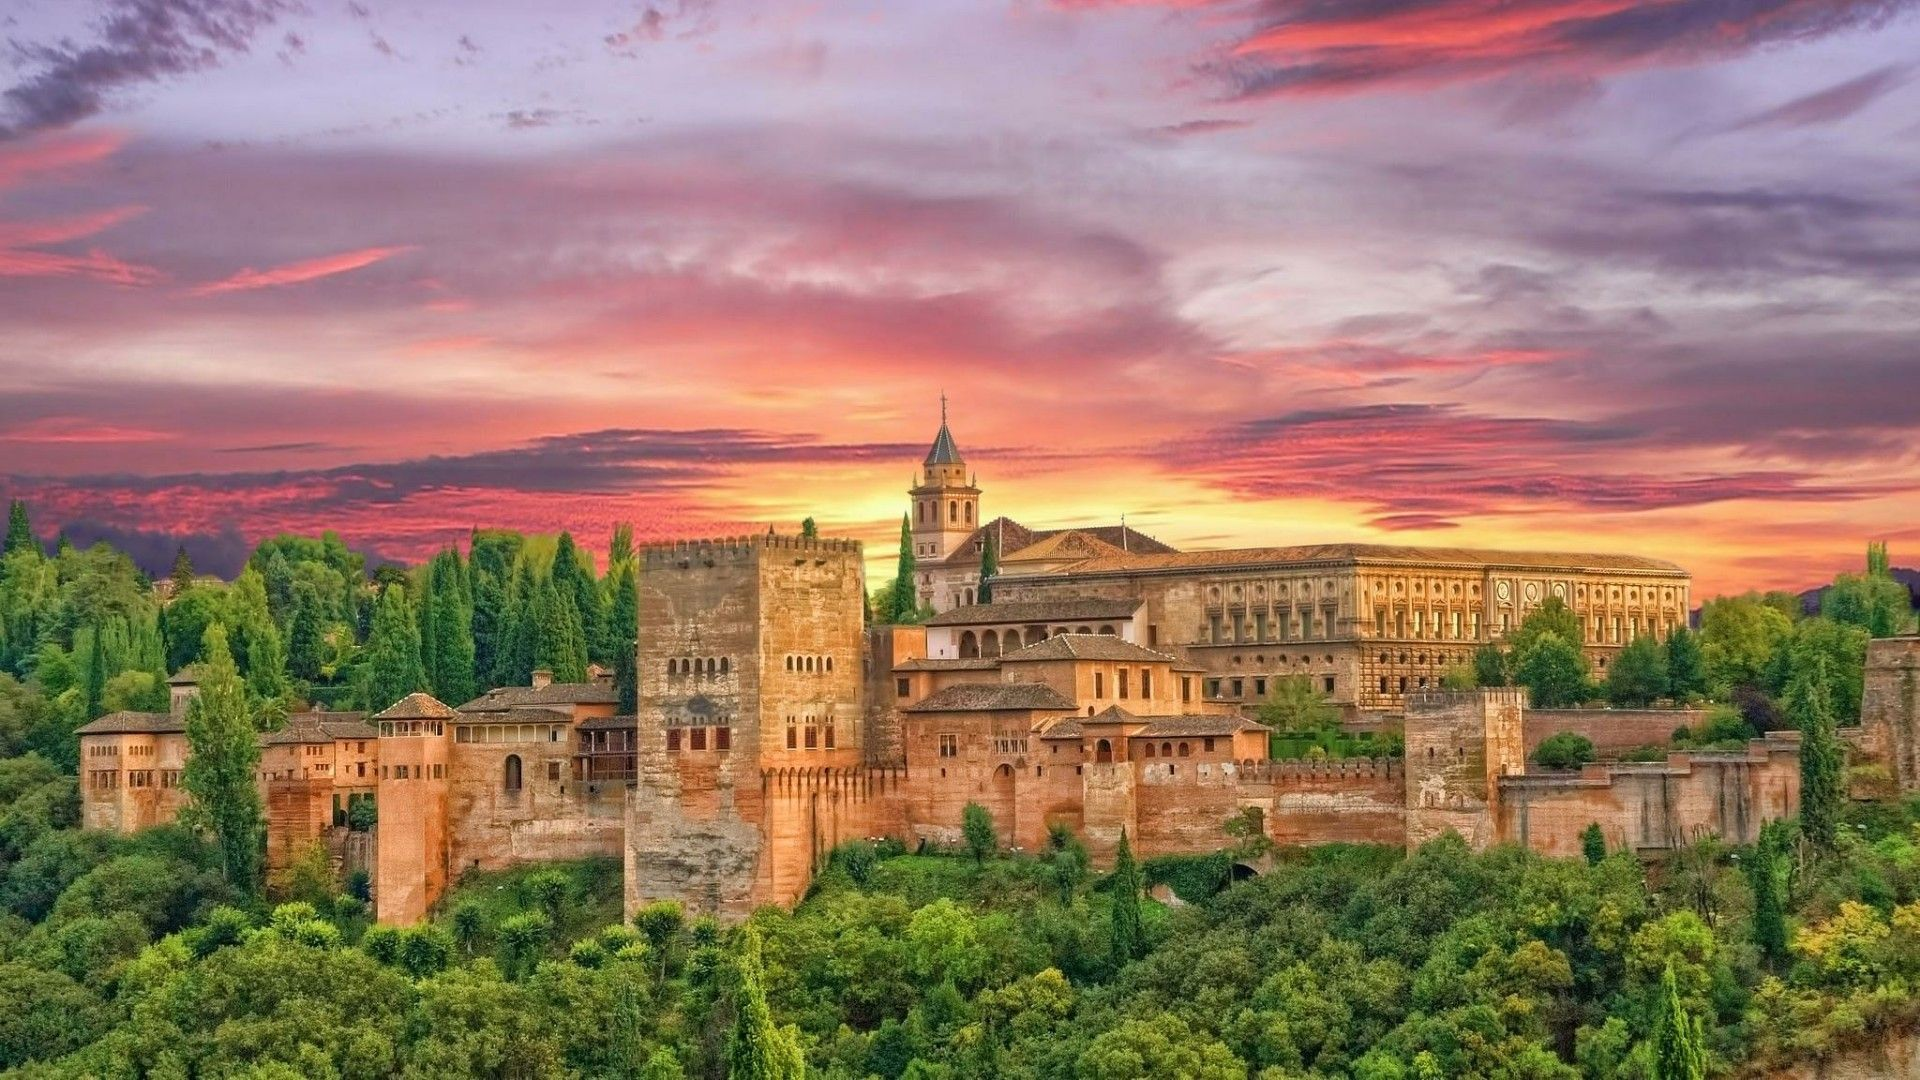
\includegraphics[width=\paperwidth,height=\paperheight,keepaspectratio]{images/granada.jpg}}
}

% Inicio del documento
\begin{document}

% Portada
\maketitle
\thispagestyle{empty}

\begin{center}
    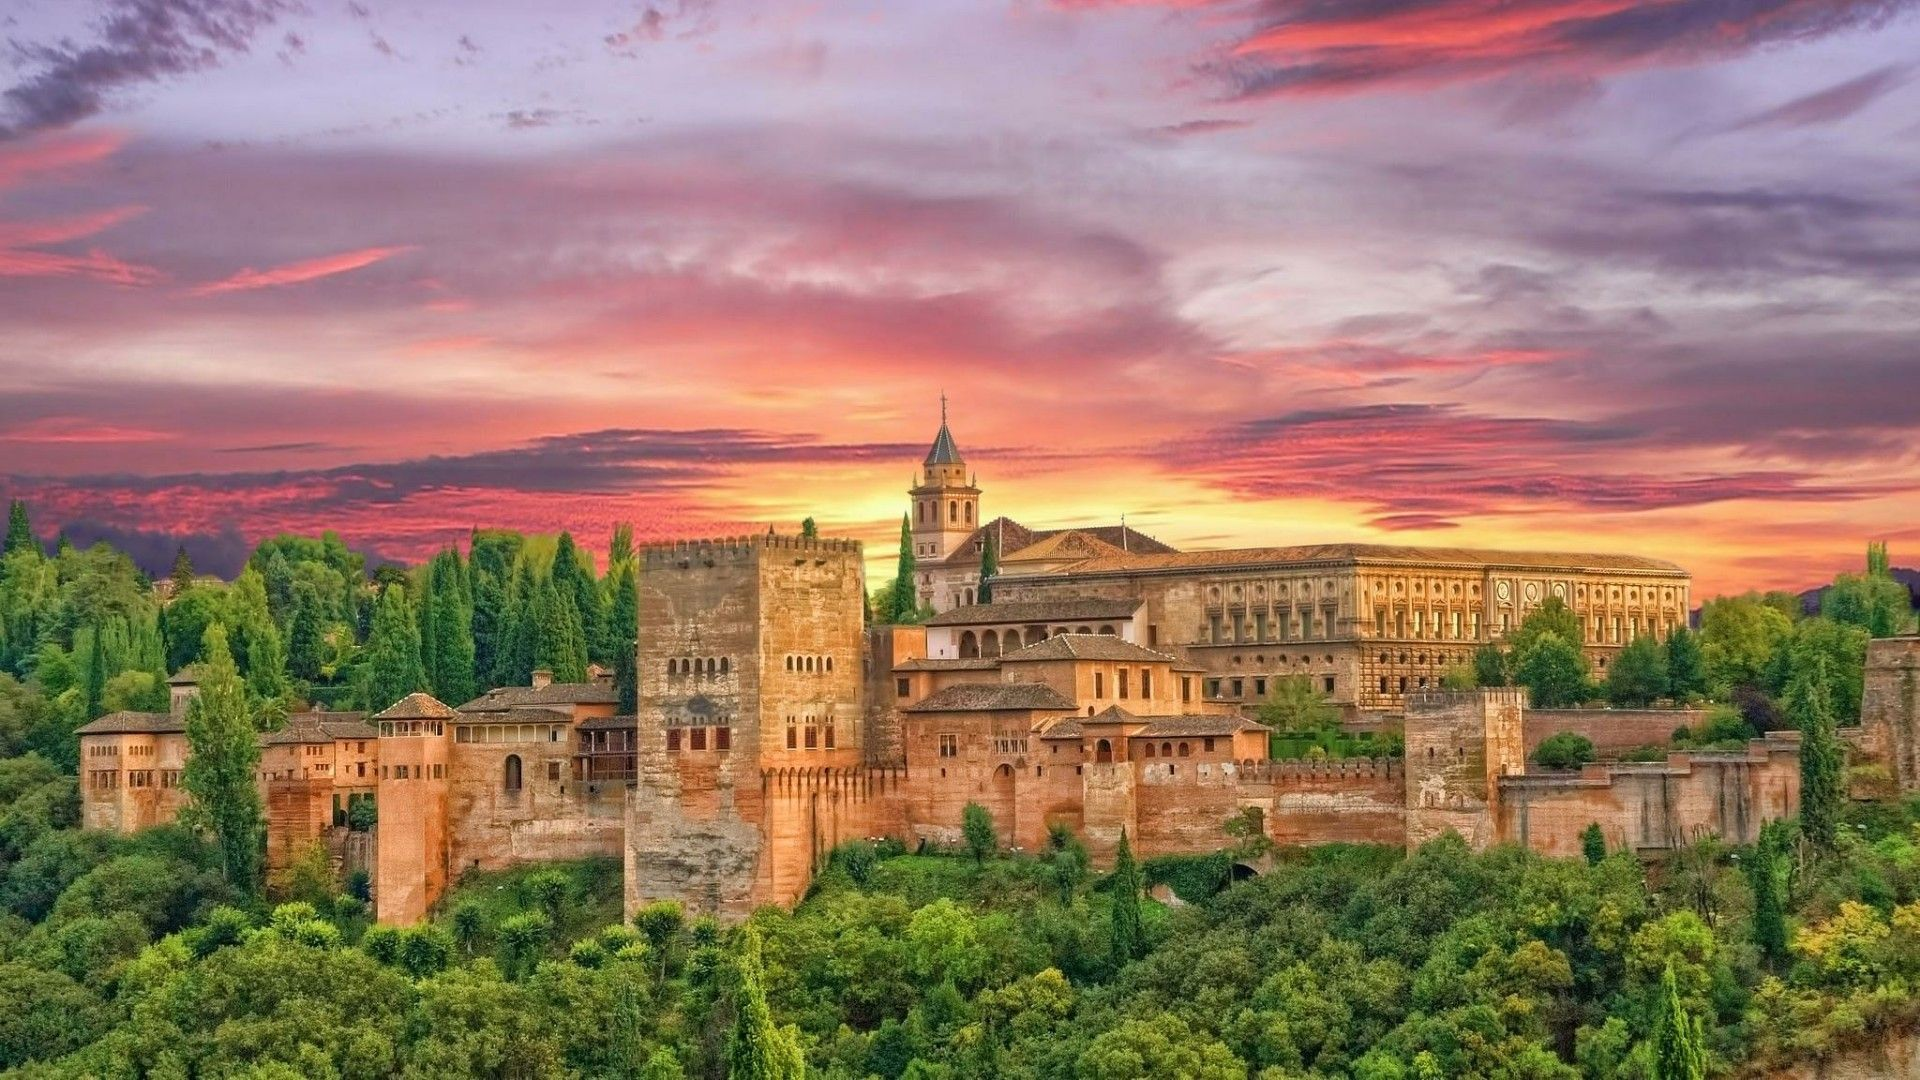
\includegraphics[width=\textwidth,height=0.4\textheight,keepaspectratio]{images/granada.jpg} \\ % Añade tu imagen de fondo
    \vfill
\end{center}

\newpage

% Índice (opcional)
\tableofcontents
\newpage

\section{Tema 2}

\subsection{Modelo Lineal Simple}

\begin{equation}
    Y_i \approx a + bx_i
\end{equation}

\subsection{Modelo Lineal Múltiple}

\begin{equation}
    Y_i = \beta_1 + \beta_2 x_{i2} + \beta_3 x_{i3} + \ldots + \beta_k x_{ik} + u_i
\end{equation}

\begin{itemize}
    \item El subíndice $i$ indica la observación.
    \item El subíndice $k$ indica el número de variables explicativas.
    \item El subíndice $u$ indica el término de error.
    \item Nota: $\beta_1$ es la constante, lleva asociado el valor 1 = $x_{i1}$ (por eso no se pone).
\end{itemize}

\subsection{Notación MLP}

\begin{equation}
    \vec{y} = \begin{pmatrix}
    Y_1 \\
    Y_2 \\
    \vdots \\
    Y_n
    \end{pmatrix}
    \end{equation}
    
    \begin{equation}
    X = \begin{pmatrix}
    1 & X_{21} & \cdots & X_{k1} \\
    1 & X_{22} & \cdots & X_{k2} \\
    \vdots & \vdots & \ddots & \vdots \\
    1 & X_{2n} & \cdots & X_{kn}
    \end{pmatrix}
    \end{equation}
    
    \begin{equation}
    \vec{\beta} = \begin{pmatrix}
    \beta_1 \\
    \beta_2 \\
    \vdots \\
    \beta_k
    \end{pmatrix}
    \end{equation}
    
    \begin{equation}
    \vec{u} = \begin{pmatrix}
    u_1 \\
    u_2 \\
    \vdots \\
    u_n
    \end{pmatrix}
    \end{equation}

\subsection{Supuestos}
\subsubsection{Linealidad}
\begin{equation}
    Y_i = \beta_1 + \beta_2 x_{i2} + \beta_3 x_{i3} + \ldots + \beta_k x_{ik} + u_i
\end{equation}

\subsubsection{Rango Completo Por Columnas}

\begin{equation}
    rango(X) = k
\end{equation}

\subsubsection{Exogeneidad}
\begin{equation}
    E(u_i|X_i) = 0
\end{equation}
\begin{itemize}
    \item El valor esperado de la esperanza que toman las variables explicativas es 0.
\end{itemize}

Por lo que si tenemos que: $Y_i = \vec{X_i^{t}}\vec{\beta}$, tenemos de forma inmediata que:
\begin{equation}
    E(Y_i|X_i) = \vec{X_i^{t}}\vec{\beta}
\end{equation}

\subsubsection{Causalidad}

\begin{itemize}
    \item Relación de causalidad es unidireccional.
    \item Las variables aparecen en el lado derecho de la ecuación, pero no al contrario.
    \item La variable dependiente $Y_i$ adoptará un carácter aleatorio.
\end{itemize}

\subsubsection{Perturbación}
\begin{itemize}
    \item Esta centrada, es decir, $E(u_i) = 0 \forall i=1,2,\ldots,n$
    \item Es homocedástica, es decir, $Var(u_i) = E[u_i^{2}]= \sigma^2 \forall i=1,2,\ldots,n$
    \item Si es incorrelada implica que $cov[u_iu_j] = E[u_iu_j]=0$. Cuando es $neq$ 0 decimos que hay un problema de autocorrelación.
\end{itemize}

Como consecuencia tenemos que:
\begin{equation}
    var[\vec{u}] = E[(\vec{u}-E[\vec{u}])(\vec{u}-E[\vec{u}])^{t}] = E[\vec{u}\vec{u}^{t}]
\end{equation}
Para la demostración de esta operación pincha \href{https://github.com/ElblogdeIsmael/ElblogdeIsmael.github.io/blob/main/Asignaturas/Tercer%20A%C3%B1o/ECO/Formulario/FCCEE/ecotema2_1.pdf}{aquí} para verla.

% diapos 28 de mi tablet teoria tema 2

\section{Tema 3}

\begin{itemize}
    
\item Varianza de las perturbaciones:
\begin{equation}
    \hat{\sigma}^2 = \frac{SCT}{n-k}
\end{equation}

\item Matriz de varianzas y covarianzas de los estimadores:
\begin{equation}
    \hat{var}(\hat{\beta}) = \hat{\sigma}^2 (X'X)^{-1}
\end{equation}

\item Hipótesis para estimar la significación individual para la constante:
\begin{align}
    H_0: \beta_{1} = 0 \\
    H_1: \beta_{1} \neq 0
\end{align}

Siendo el estadístico experimental:
\begin{equation}
    t_{exp} = \frac{\hat{\beta_1}}{\sqrt{\hat{var}(\hat{\beta_1})}} ; t_{teorico} = t_{n-k,1-\frac{\alpha}{2}}
\end{equation}

\item Para la tabla ANOVA el F experimental es:
\begin{equation}
    F_{exp} = \frac{SCE/k-1}{SCR/n-k} ; F_{teorico} = F_{k-1,n-k,1-\alpha}
\end{equation}

\item Intervalo de confianza para los estimadores y la varianza de la perturbación.
En este caso vamos a usar una notación distinta a la de la teoría para simplificar la interpretación:
\begin{itemize}
\item IC para los estimadores
\begin{equation}
    \beta_i \in (\hat{\beta_i} \pm t_{n-k, 1-\frac{\alpha}{2}} \cdot \sqrt{M_{ii}})
\end{equation}

Siendo $M_{ii}$ la matriz $\hat{\sigma}^{2}(XX^{\prime})$ en la posición $i,i$.

\item IC para la varianza de la perturbación
\begin{equation}
    \frac{(n-k)\hat{\sigma^2}}{\chi^2_{n-k}(\frac{\alpha}{2})};\frac{(n-k)\hat{\sigma^2}}{\chi^2_{n-k}(\frac{1-\alpha}{2})}
\end{equation}

\end{itemize}

\item Sabiendo el valor del $R^2$, contrastar la significación global del modelo:

\begin{equation}
    \frac{\frac{R^2}{k-1}}{\frac{1-R^2}{n-k}} \sim F_{k-1,n-k}(1-\alpha)
\end{equation}


\end{itemize}


\end{document}
